% \pagebreak[4]
% \hspace*{1cm}
% \pagebreak[4]
% \hspace*{1cm}
% \pagebreak[4]

\chapter{Giới Thiệu }
\ifpdf
    \graphicspath{{Chapter1/Chapter1Figs/PNG/}{Chapter1/Chapter1Figs/PDF/}{Chapter1/Chapter1Figs/}}
\else
    \graphicspath{{Chapter1/Chapter1Figs/EPS/}{Chapter1/Chapter1Figs/}}
\fi

%\begin{quote}
%\textit{Nhận dạng hành động người là một trong những hướng nghiên cứu thách thức nhất trong lĩnh vực thị giác máy tính. Trong chương này khóa luận tập trung giới thiệu tổng quan về bài toán, làm sáng tỏ động lực nghiên cứu cũng như các thách thức còn tồn đọng. Cuối cùng, bố cục nội dung trình bày trong khóa luận sẽ được tóm tắt ở phần kết của chương.}
%\end{quote}

Trong những năm gần đây, phương pháp học có giám sát của máy học đã được áp dụng để giải quyết nhiều bài toán trong thị giác máy tính, xử lý âm thanh, xử lý ngôn ngữ tự nhiên, … Thông thường, từ dạng biểu diễn thô ban đầu (ví dụ như ma trận pixel), ta cần phải chuyển sang một dạng biểu diễn tốt hơn, có nhiều ngữ nghĩa hơn – gọi là \emph{biểu diễn đặc trưng} (feature representation); rồi mới đưa dạng biểu diễn đặc trưng này vào một thuật toán học có giám sát (ví dụ như SVM). Việc xác định cách biểu diễn đặc trưng đóng vai trò rất quan trọng để thuật toán học giám sát có thể thực hiện hiệu quả. 

Để xác định cách biểu diễn đặc trưng, hướng tiếp cận truyền thống là \emph{thiết kế đặc trưng một cách thủ công} (hand-designed features). Nghĩa là với một lĩnh vực cụ thể, sẽ có những nhóm nghiên cứu gồm các chuyên gia trong lĩnh vực đó cùng ngồi xuống, phân tích, thiết kế, ``thử và sai'' các cách biểu diễn đặc trưng từ dạng biểu diễn thô ban đầu. Ví dụ về các đặc trưng được thiết kế thủ công trong thị giác máy tính là SIFT, HOG, SURF, …; trong xử lý âm thanh là Spectrogram, MFCC, Spectral rolloff, … Tuy nhiên, nhược điểm của hướng tiếp cận này là tốn thời gian và tốn sức lao động; đồng thời cũng thiếu tính tổng quát hóa: các đặc trưng này chỉ sử dụng được cho một loại dữ liệu cụ thể (ví dụ, đặc trưng SIFT chỉ sử dụng được cho một số loại ảnh cụ thể trong thị giác máy tính). Ngoài ra, việc thiết kế đặc trưng một cách thủ công như trên cũng cho thấy điểm yếu của các thuật toán máy học hiện nay: thiếu khả năng tự động rút trích các thông tin có ích trực tiếp từ dữ liệu thô ban đầu.

Do đó, thay vì thiết kế các trưng một cách thủ công, ta mong muốn có một thuật toán có thể \emph{tự động học các đặc trưng} từ dữ liệu thô ban đầu. Hơn nữa, ta mong muốn tìm được một thuật toán mà có thể áp dụng tổng quát cho nhiều loại dữ liệu (hình ảnh, âm thanh, …). Ngoài ra, ta muốn học các đặc trưng từ tập dữ liệu không có nhãn (unlabeled data) vì dữ liệu không có nhãn có rất nhiều; trong khi đó, dữ liệu có nhãn không có nhiều và phải tốn chi phí để có thể có thêm. Hướng nghiên cứu này được gọi là \emph{học đặc trưng không giám sát} (unsupervised feature learning). Đây là một hướng nghiên cứu mới trong máy học và đang thu hút được rất nhiều sự quan tâm trong thời gian gần đây.

Để giải quyết bài toán học đặc trưng không giám sát, câu hỏi lớn và mang tính định hướng nghiên cứu dài hạn là: \emph{Thế nào là một biểu diễn đặc trưng tốt?} Theo GS. Yoshua Bengio, một trong những nhà nghiên cứu tiên phong trong lĩnh vực học biểu diễn đặc trưng, thì: \emph{Một biễu diễn đặc trưng tốt cần \textbf{phân tách (disentangle)} được các yếu tố giải thích ẩn bên dưới} \cite{bengio2013representation}. Hình \ref{fig_disentangle} minh họa cho điểm này; ở đây, chó, mèo, cây, ... là các yếu tố giải thích cho bức ảnh và một biểu diễn đặc trưng tốt cần tìm ra được các yếu tố giải thích này. 

\begin{figure}
	\centering
	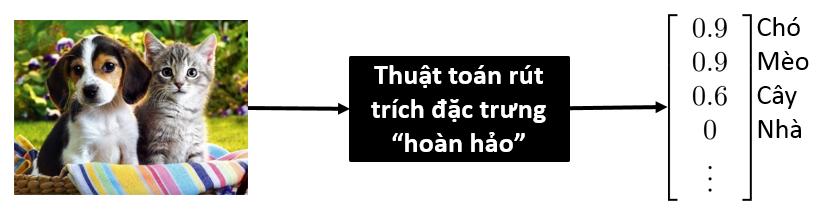
\includegraphics[width=\textwidth]{disentangle}
	\caption[Minh họa về một biểu diễn đặc trưng tốt]{Minh họa về một biểu diễn đặc trưng tốt: phân tách được các yếu tố giải thích ẩn bên dưới (chó, mèo, cây, ...)}
	\label{fig_disentangle}
\end{figure}

Cho đến nay, vẫn chưa có một thuật toán học đặc trưng mà có thể phân tách tốt được các yếu tố giải thích ẩn bên dưới. Để có thể phân tách được các yếu tố giải thích ẩn, ta cần có \emph{các sự hiểu biết trước (priors)} về các yếu tố này. Ở đây, ta quan tâm đến các sự hiểu biết trước mang tính tổng quát, có thể áp dụng để học đặc trưng trong nhiều bài toán liên quan đến trí tuệ nhân tạo (thị giác máy tính, xử lý ngôn ngữ tự nhiên, ...). Dưới đây là một số sự hiểu biết trước như vậy \cite{bengio2013representation}:
\begin{itemize}
	\item \textbf{Các yếu tố giải thích được tổ chức một cách phân cấp}: Thế giới xung quanh ta có thể được mô tả bằng một kiến trúc phân cấp. Cụ thể là, các yếu tố hay các khái niệm (concept) trừu tượng (ví dụ như con mèo, cái cây, ...) bao gồm các khái niệm ít trừu tượng hơn; các khái niệm ít trừu tượng hơn này lại bao gồm các khái niệm ít trừu tượng hơn nữa ... \emph{Học sâu (deep learning)} sử dụng sự hiểu biết này: học nhiều tầng biểu diễn đặc trưng với độ trừu tượng tăng dần.
	\item \textbf{Gom cụm tự nhiên (natural clustering)}: các mẫu thuộc các lớp khác nhau nằm trên các đa tạp (manifold) khác nhau và các đa tạp này được phân tách tốt với nhau bởi các vùng có mật độ thấp; hơn nữa, số chiều của các đa tạp này nhỏ hơn rất nhiều so với số chiều của không gian ban đầu.
	\item \textbf{Tính thưa (sparsity)}: với mỗi mẫu dữ liệu (ví dụ, với mỗi bức ảnh), chỉ có một số ít các khái niệm (hay các yếu tố giải thích) trong tập các khái niệm. Do đó, với mỗi mẫu dữ liệu, ta muốn tìm một véc-tơ biểu diễn \emph{thưa}, nghĩa là hầu hết các phần tử của véc-tơ này có giá trị bằng 0 (ứng với các khái niệm không liên quan trong tập khái niệm).
\end{itemize}

Trong luận văn này, chúng tôi sẽ tập trung nghiên cứu về tính thưa. Việc tích hợp tất cả các hiểu biết trước ở trên (cũng như là tìm ra thêm các hiểu biết trước mới) vào trong cùng một mô hình sẽ có thể giúp phân tách các yếu tố giải thích ẩn tốt hơn, nhưng đây là một điều không đơn giản và chúng tôi để lại như là một định hướng cho việc nghiên cứu trong tương lai. Tính thưa lần đầu tiên được đề xuất trong thuật toán ``Sparse Coding'' \cite{olshausen1996emergence} để mô hình vùng vỏ não thị giác V1 (là vùng đầu tiên xử lý tín hiệu thị giác từ võng mạc mắt). Và điểm thú vị là ``Sparse Coding'' có thể học được những đặc trưng tương tự như những đặc trưng của vùng V1 (có dạng các cạnh ở các vị trí khác nhau và với các hướng khác nhau).

``Sparse Auto-Encoders'' (SAEs) có thể học được các đặc trưng giống với ``Sparse Coding''. Tuy nhiên, so với ``Sparse Coding'', SAEs có những điểm lợi như sau:
\begin{itemize}
	\item Việc huấn luyện SAEs có thể được thực hiện một cách hiệu quả với thuật toán lan truyền ngược (back-propagation).
	\item Sau khi đã được huấn luyện, với một véc-tơ đầu vào mới, SAEs có thể tính ra véc-tơ đặc trưng tương ứng rất nhanh; trong khi đó, ``Sparse Coding'' vẫn phải tiến hành tối ưu hóa.
	\item Sau khi đã học đặc trưng không giám sát, SAEs có thể cho phép điều chỉnh lại (fine-tune) các đặc trưng này với các mẫu huấn luyện có nhãn. Nhìn chung, việc điều chỉnh này thường sẽ cho kết quả tốt hơn so với việc không điều chỉnh.
\end{itemize}

Tuy có những lợi điểm trên, nhưng trong thực tế thì không dễ để làm cho SAEs ``hoạt động''. Để làm cho SAEs ``hoạt động'', có hai điểm cần phải làm rõ: (i) ràng buộc thưa, và (ii) ràng buộc trọng số. Sử dụng chuẩn L1 để ràng buộc tính thưa của véc-tơ đặc trưng là một cách tự nhiên (vì L1 được dùng trong ``Sparse Coding'') và đơn giản (trong trường hợp véc-tơ đặc trưng có giá trị dương, L1 đơn giản là bằng tổng của các phần tử của véc-tơ này), nhưng L1 lại thường không được dùng trong SAEs với lý do vẫn còn chưa rõ ràng \cite{bengio2013representation}. Thay vì dùng L1, các nghiên cứu liên quan đến SAEs thường ràng buộc thưa bằng cách ép giá trị đầu ra trung bình của mỗi nơ-ron ẩn (trong SAEs, mỗi nơ-ron ẩn ứng với một đặc trưng) về một giá trị cố định gần 0 \cite{goodfellow2009measuring}\cite{coates2011analysis}\cite{coates2012demystifying}. Tuy nhiên, giá trị cố định này lại thêm một siêu tham số (hyper-parameter, là tham số mà ta phải chọn trước khi huấn luyện) vào danh sách các siêu tham số vốn đã rất nhiều của SAEs; điều này sẽ làm cho quá trình chọn lựa các siêu tham số trở nên rất ``phiền phức'' và tốn thời gian. Về vấn đề ràng buộc trọng số của SAEs, có một số cách khác nhau đã được sử dụng. \cite{coates2012demystifying} ràng buộc các trọng số của bộ mã hóa (encoder) giống với các trọng số của bộ giải mã (decoder). Cách ràng buộc trọng số này cũng được dùng cho các loại ``Auto-Encoders'' khác như ``Denoising Auto-Encoders'' \cite{vincent2008extracting} và ``Contractive Auto-Encoders'' \cite{rifai2011contractive}\cite{rifai2011HCAEs}. \cite{goodfellow2009measuring}\cite{coates2011analysis} dùng một cách ràng buộc trọng số khác là ``weight decay'' (phạt tổng bình phương các trọng số); cách này lại làm xuất hiện thêm một siêu tham số nữa. \cite{zeiler2013rectified} ràng buộc các véc-tơ trọng số của tầng giải mã (mỗi véc-tơ ứng với các trọng số đi ra ở mỗi nơ-ron ẩn) có độ dài bằng một. Tuy nhiên, trong số các cách ràng buộc trọng số này, không rõ là nên sử dụng cách nào cũng như là tại sao nên ràng buộc các trọng số như vậy.

Như vậy, có hai câu hỏi cần phải được trả lời: (i) tại sao chuẩn L1 lại thường không được dùng để ràng buộc thưa trong SAEs?; (ii) liệu có cách nào tốt hơn và hợp lý hơn để ràng buộc trọng số của SAEs không? Trong luận văn này, chúng tôi sẽ cố gắng trả lời hai câu hỏi này. Cụ thể là:
\begin{itemize}
	\item Chúng tôi cố gắng hiểu khó khăn của việc huấn luyện SAE với ràng buộc thưa dùng chuẩn L1. Từ đó, chúng tôi đề xuất một phiên bản điều chỉnh của thuật toán tối ưu hóa ``Stochastic Gradient Descent'' (SGD), gọi là ``Sleep-Wake Stochastic Gradient Descent'' (SW-SGD), để giải quyết khó khăn này. Ở đây, chúng tôi tập trung nghiên cứu SAEs với hàm kích hoạt ở tầng ẩn là hàm ``rectified linear'' ($f(x) = \max(0, x)$) bởi vì hàm này tính nhanh và cho tính thưa thật sự (đúng bằng 0). Chúng tôi gọi SAEs với hàm kích hoạt này là \emph{``Sparse Rectified Auto-Encoders''} (SRAEs).
	\item Hơn nữa, chúng tôi cũng đề xuất một cách hợp lý để ràng buộc trọng số của SRAEs.
\end{itemize}

Với hai thành phần trên (SW-SGD và cách ràng buộc trọng số mà chúng tôi đề xuất), kết quả thí nghiệm trên bộ dữ liệu MNIST (bộ dữ liệu chữ số viết tay từ 0 đến 9) cho thấy SRAEs có thể học được những đặc trưng có ích và những đặc trưng này cho kết quả phân lớp tốt khi so sánh với các loại ``Auto-Encoders'' khác.

Phần còn lại của luận văn được trình bày như sau:
\begin{itemize}
	\item Chương 2 trình bày kiến thức nền tảng về ``Sparse Coding'' và ``Sparse Auto-Encoders''.
	\item Chương 3 trình bày về ``Sparse Rectified Auto-Encoders'' (SRAEs); đây là phần chính của luận văn. Trong phần này gồm có hai phần nhỏ:
	\begin{itemize}
		\item Ràng buộc thưa: chúng tôi giải thích về vấn đề gặp phải khi huấn luyện SRAEs với chuẩn L1 và đưa ra giải pháp để giải quyết vấn đề này.
		\item Ràng buộc trọng số: chúng tôi trình bày về cách ràng buộc trọng số đề xuất cho SRAEs.
	\end{itemize}
	\item Chương 4 trình bày về các thí nghiệm và các phân tích về kết quả đạt được.
	\item Cuối cùng, kết luận và hướng phát triển được trình bày ở chương 5.
\end{itemize}